\documentclass{standalone}

% Fonts
\usepackage[T1]{fontenc}
\usepackage[utf8]{inputenc}
\usepackage{newpxtext,newpxmath}
\usepackage{sectsty}

\usepackage{xcolor}
\usepackage{tikz}
\usetikzlibrary{arrows.meta,calc,positioning}
\usetikzlibrary{shapes.multipart, arrows.meta, positioning, matrix}
\usetikzlibrary{trees}
\usetikzlibrary{trees}
\usepackage{pgfplots}
\pgfplotsset{compat=1.17}
\usepackage{pgfgantt}
% define your status‐styles once
\tikzset{
	notstarted/.style = {circle,draw,fill=gray!20,minimum size=6mm,inner sep=0pt},
	inprogress/.style = {circle,draw,fill=yellow!60,minimum size=6mm,inner sep=0pt},
	done/.style        = {circle,draw,fill=green!60,minimum size=6mm,inner sep=0pt},
	snake it/.style={decorate, decoration=snake},
}

\begin{document}
	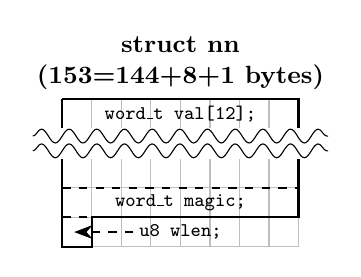
\begin{tikzpicture}[x=1cm, y=-0.05cm, font=\scriptsize, draw=black, >=Stealth, scale=.75]
		\draw[gray!50, step=0.5cm] (0,0) grid (4, 50);
%		\draw[thick] (0,0) rectangle ++(4,60);  % 128 bytes tall, 3 cm wide
		\draw[thick] (0,0) -- ++(0,50) -- ++(.5,0) -- ++(0,-10) -- ++(3.5,0) -- ++(0,-40) -- ++(-4,0);
		\filldraw[white] (-.5,10) rectangle (4.5, 20);
		\draw[snake it] (-.5,12.5) -- (4.5,12.5);
		\draw[snake it] (-.5,17.5) -- (4.5,17.5);
		% BlockCipherContext labels and offsets
		\node[anchor=south, align=center, font=\small] at (2,0) {\textbf{struct nn}\\ \textbf{(153=144+8+1 bytes)}};
		\node[align=center] at (2,5) {\texttt{word\_t val[12];}};
		\node[align=center] at (2,35) {\texttt{word\_t magic;}};
		\draw[thick, dashed] (0,30) -- ++(4,0);
		\draw[thick, dashed] (0,40) -- ++(.5,0);
		\node[align=center] at (2,45) {\texttt{u8 wlen;}};
		\draw[thick, dashed, -Stealth] (1.2,45) -- ++(-1,0);
	\end{tikzpicture}
\end{document}